\section{Mesure des performances}
\label{efficacite}
Dans cette dernière partie nous allons appliquer les différent algorithmes sur un grand nombre d'instances de test contenant chacune 256 points. Cela nous permettra de faire une moyenne sur le temps d'exécution mais aussi sur l'efficacité des conteneurs que sont le rectangle et le cercle par rapport au polygone convexe qui est la plus optimale.

La formule calculant l'efficacité en \%, c'est-à-dire dans quelle proportion est-ce que l'aire du conteneur est plus grand que l'aire de l'enveloppe convexe), est la suivante :
\begin{equation}
\textrm{qualité} = \left( \frac{\textrm{aire}}{\textrm{aire polygone}} \times 100\right) - 100
\end{equation}

Pour calculer l'aire du polygone, nous nous servons de la formule suivante (donnée en \cite{mathwords}) :
\begin{equation}
\textrm{aire polygone} = \frac{1}{2} \begin{vmatrix}
x_1 & y_1 \\
x_2 & y_2 \\
x_3 & y_3 \\
\vdots & \vdots \\
x_n & y_n \\
x_1 & y_1
\end{vmatrix}
\label{aire}
\end{equation}

La formule \eqref{aire} est également utilisée pour calculer l'aire du rectangle. Quand à l'aire du cercle, nous nous servons tout simplement de la formule :
\begin{equation}
\textrm{aire cercle} = \pi r^2
\end{equation}
\subsection{Résultats}
Nous allons ici présenter les résultats obtenus en expérimentant les algorithmes de Toussaint et de Ritter avec 1663 instances de test de la base VAROUMAS fournis. Les algorithmes ont été exécutés sur un ordinateur équipé de 12GB RAM et d'un processeur \textit{Intel Core i7 4790K} cadencé à 4.00GHz tournant sous \textit{Windows 10 Pro 64-bit}.

\begin{center}
\begin{tabular}{|*{4}{c|}}
    \hline
       & Graham  & Toussaint  & Ritter \\
    \hline
     Temps min.  & 0.025103 ms  &0.25538 ms  & 0.009989 ms \\
    \hline
     Temps moy.  & 0.039666 ms  & 0.306384 ms  & 0.019886 ms \\
    \hline
     Temps max.  & 1.697752 ms  & 6.256938 ms & 1.028693 ms \\
    \hline
\end{tabular}
\captionof{table}{Temps d'exécution}
\label{texec}
\end{center}

\begin{figure}[ht]
\begin{center}
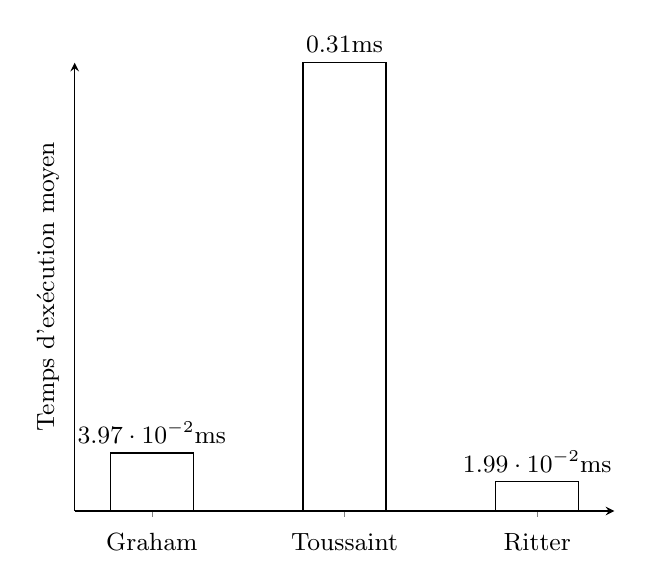
\begin{tikzpicture}[font=\small]
    \begin{axis}[
      ybar,
      bar width=30pt,
      ylabel={Temps d'exécution moyen},
      ymin=0,
      ytick=\empty,
      xtick=data,
      axis x line=bottom,
      axis y line=left,
      enlarge x limits=0.2,
      symbolic x coords={Graham, Toussaint,Ritter},
      xticklabel style={anchor=base,yshift=-\baselineskip},
      nodes near coords={\pgfmathprintnumber\pgfplotspointmeta ms}
    ]
      \addplot[fill=white] coordinates {
      	(Graham,0.039666)
        (Toussaint,0.306384)
        (Ritter,0.019886)
      };
    \end{axis}
\end{tikzpicture}
\label{gtime}
\end{center}
\end{figure}

\begin{center}
\begin{tabular}{|*{3}{c|}}
    \hline
       & Toussaint  & Ritter \\
    \hline
     Efficacité  & 25,23\%  & 20,52\%  \\
    \hline
\end{tabular}
\captionof{table}{Efficacité}
\label{eff}
\end{center}

\begin{figure}[ht]
\begin{center}
\begin{tikzpicture}[font=\small]
    \begin{axis}[
      ybar,
      bar width=30pt,
      ylabel={Efficacité},
      ymin=0,
      ytick=\empty,
      xtick=data,
      axis x line=bottom,
      axis y line=left,
      enlarge x limits=0.2,
      symbolic x coords={Toussaint,Ritter},
      xticklabel style={anchor=base,yshift=-\baselineskip},
      nodes near coords={\pgfmathprintnumber\pgfplotspointmeta\%}
    ]
      \addplot[fill=white] coordinates {
        (Toussaint,25.23)
        (Ritter,20.52)
      };
    \end{axis}
\end{tikzpicture}
\label{geff}
\end{center}
\end{figure}
\subsection{Interprétation}
D'après les résultats obtenus, on remarque que l'algorithme de Toussaint prend largement plus de temps à s'exécuter par rapport à l'algorithme de Ritter. En effet, nous avions vu que l'algorithme de Toussaint était pseudo-linéaire, dû au parcours préliminaire de Graham, alors que celui de Ritter est linéaire. Dans un cas défavorable, on peut même observer que l'algorithme de Toussaint est 6 fois plus long en exécution que celui de Ritter.

En terme d'efficacité, l'algorithme de Ritter est également plus optimale puisque que la superficie du cercle minimum est en moyenne 20.52\% plus grand que celle de l'enveloppe convexe, contre 25.35\% pour le rectangle minimum.

On pourrait prendre d'autres critères d'évaluation que le temps d'exécution ou l'efficacité comme la complexité mémoire par exemple, qui serait elle aussi à l'avantage de l'algorithme de Ritter étant donné que celui de Toussaint requiert la conservation en mémoire de beaucoup plus de paramètres.

\paragraph{}
Tout porte à croire que l'algorithme de Ritter est largement préférable à celui de Toussaint, pour en être sûr il aurait fallu expérimenter sur un plus large éventail de test que celui de VAROUMAS et sur des instances plus grandes : 256 points constitue en effet une instance de taille relativement petite.

En revanche, pour en revenir au temps d'exécution, l'algorithme de Toussaint semble être un bon candidat à la parallélisation. En effet, on pourrait répartir les calculs de chaque rectangle et les exécuter en parallèle avant de finalement comparer leur superficie, contrairement à l'algorithme de Ritter qui n'est pas parallélisable puisque c'est un algorithme glouton. Si cette parallélisation s'avère efficace, le temps d'exécution moyen s'en trouverait largement réduit même si le parcours de Graham est toujours présent dont le temps d'exécution est supérieur à Ritter.